\Chapter{REVUE DE LITTÉRATURE}\label{sec:RevLitt}
% Texte / Text.

\section{Les complexités de développer ERP}
% TODO voir article erp en entreprise
% REF implantation d’un ERP en PME

Le développement d’une solution ERP doit supporter plusieurs niveaux~\cite{uqam_erp_benefice_2008} : 
\begin{enumerate}
    \item Évaluation des besoins;
    \item Préparation du projet;
    \begin{enumerate}
        \item Organisation du projet;
        \item Définir les objectifs;
        \item Créer un plan détaillé;
    \end{enumerate}
    \item Dessin d’affaires;
    \begin{enumerate}
        \item Analyser les processus d’affaires actuels;
        \item Maîtrise du système ERP;
        \item Revue des processus;
    \end{enumerate}
    \item Réalisation;
    \begin{enumerate}
        \item Développement technique;
        \item Étude pilote;
    \end{enumerate}
    \item Préparation finale;
    \begin{enumerate}
        \item Réglages et tests;
        \item Éduquer et former la masse critique;
    \end{enumerate}
    \item Mise en production et support;
    \begin{enumerate}
        \item Déploiement des modules ERP;
        \item Améliorer et élargir les systèmes ERP de façon continue;
    \end{enumerate}
\end{enumerate}

Autour de ça, il faut mettre en place une gestion du changement et adapter le développement des affaires.

Plusieurs de ces étapes ne sont pas prises au sérieux, tel que le financement. De plus, l’implantation se fait sur une longue période de temps.

Dans Odoo, le nombre de modules augmente avec le temps et diffère entre les versions, une recherche fastidieuse doit être effectué pour réduire le temps de développement à éviter de réinventer la roue.

Il faut adapter les processus des organisations aux fonctionnalités existantes, sinon il est trop coûteux de tout recréer selon les processus de l’entreprise.

En plus de suivre toutes ces étapes, il faut mettre en place une pérennité pour l’amélioration continue sur le projet, ça devient un processus lourd qui doit durer dans le temps.


\section{Logiciel no-code / low-code}

Logiciel no-code / low-code = LCNC

Basé sur des templates de code et un interface qui permet au besoin la configuration par du code.

C’est un concept qui permet à l’utilisateur de développer une plateforme en utilisant pas ou peu de code.

% TODO REF A. C. Bock, U. Frank: Low-Code Platform, Bus Inf Syst Eng 63(6):733–740 (2021)
% TODO REF Supporting the understanding and comparison of low-code development platforms

Besoin de : 
\begin{enumerate}
    \item Aspect général;
    \begin{enumerate}
        \item Gestion des rôles et permissions par des groupes utilisateurs ou individuelle;
        \item Mécanisme de déploiement et exportation;
    \end{enumerate}
    \item Perspective d’intéraction;
    \begin{enumerate}
        \item Mécanisme pour changer le design de l’interface utilisateur;
        \item Mécanisme pour coupler l’interface à un modèle et un contrôleur (MVC);
        \item Mécanisme pour faire le rendu visuel sur différents types d’appareils;
    \end{enumerate}
    \item Perspective dynamique;
    \begin{enumerate}
        \item Gestion des processus du système et de la machine;
        \item Composantes de modélisation de processus conceptuel;
        \item Système de gestion des états et des transitions;
    \end{enumerate}
    \item Perspective fonctionnelle;
    \begin{enumerate}
        \item Mécanisme de spécification fonctionnel de base;
        \item Générateur d’algorithme;
        \item Générateur de code de composantes;
        \item Mécanisme d’accès à des API externe;
    \end{enumerate}
    \item Perspective statique;
    \begin{enumerate}
        \item Composante de conception d’un modèle de données;
        \item Composante pour spécifier des structures de données;
        \item Gestion de base de données interne;
        \item Gestion de base de données externes par API;
    \end{enumerate}
\end{enumerate}

Pour supporter une plateforme LCNC :
\begin{enumerate}
    \item Bases de données;
    \item Services externes;
    \item Gestion des modèles de données;
    \item Plateforme collaborative;
    \item Service infonuage (déploiement, audit de performance, gestion des erreurs/traces/événements, gestion des versions);
    \item Générateur de code;
    \item Compilateur et optimiseur de code;
    \item Modeleur d’application;
    \begin{enumerate}
        \item Widget;
        \item Connecteur;
        \item Processus de logique métier;
        \item Capacité de «drag and drop»;
        \item Modèle de données;
        \item Règles de sécurité;
    \end{enumerate}
\end{enumerate}
Critère de qualité d’une plateforme LCNC :
\begin{enumerate}
    \item GUI;
    \item Interoperability support entre services externes et base de données;
    \item Support de la sécurité;
    \item Support d’une plateforme collaborative;
    \item Support sur la réusabilité, pouvoir répété l’utilisation d’une composante dans différents contextes;
    \item Support de la capacité d’un système à maintenir ou à améliorer ses performances;
    \item Mécanisme de spécification de logique du développement des affaires;
    \item Logiciel pour construire des mécanismes;
    \item Support au déploiement;
\end{enumerate}

\section{Génération de code}
TODO

\section{Logiciel Open Source}
Actuellement, une méthode utilisée pour accélérer le développement est le partage de bibliothèque, une fonctionnalité aurait déjà été programmé et le rendre accessible publiquement permet la réduction d’écriture du code pour réaliser une fonctionnalité souhaitée.

L’Open Source permet aussi de supporter l'interopérabilité~\cite{open_interop_2011}, c’est la capacité de différents logiciels d'interagir et communiquer efficacement entre eux sans entraves ni obstacles, il permet à différents systèmes de fonctionner ensemble de manière transparente et harmonieuse même s’ils ont été développés par différentes organisations.

% \section{Logiciel Libre}
% Le logiciel libre entrave l’interopérabilité seulement pour les systèmes non compatibles avec la copyleft. Bien qu’elle prône la liberté du code, elle est restrictive.

% Cette restriction est nécessaire à la protection du développeur et de la communauté. 

% \section{Dev ops}
% Démontrer outil
% TODO image dev ops

% La partie générateur de code répond seulement au besoin création de code du dev ops.

\section{Création d’une communauté}

\subsection{Communication non violente}

Réduire les frictions entre les participants du réseau d’entraide. C’est avec la mise en place d’une méthode de communication non violente~\footnote{\url{https://fr.wikipedia.org/wiki/Communication_non_violente}} formalisée par Marshall B. Rosenberg, voir Figure~\ref{fig:communication_non_violente}.

\begin{figure}[htb]
\centering
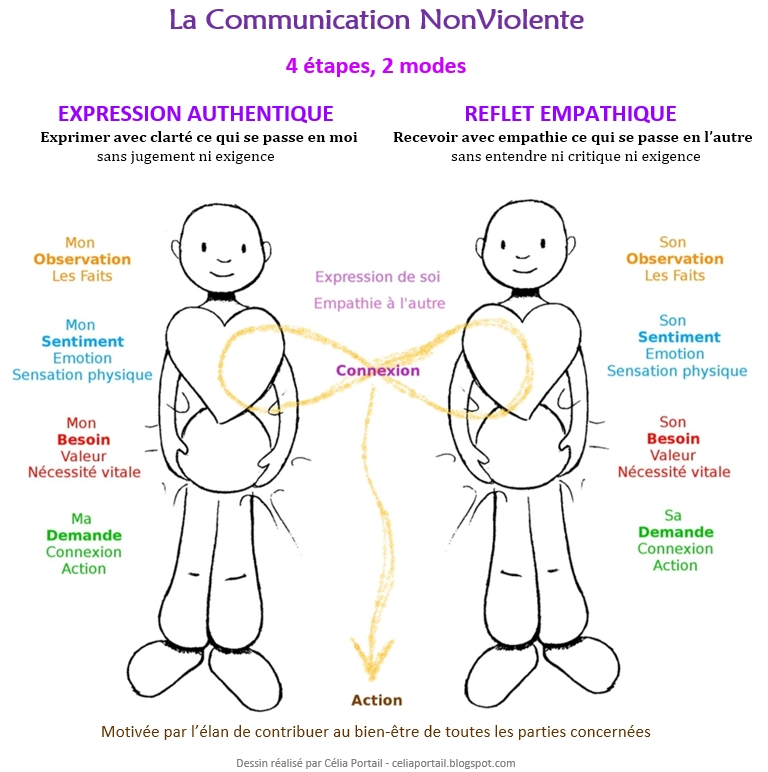
\includegraphics[width=4in]{OSBD_en_CNV.jpg}
\caption{Communication non violente en 4 étapes et 2 modes}
\label{fig:communication_non_violente}
\end{figure}

\subsection{Guide construire une communauté Open Source}
Guide en 4 sections avec des titres indicateurs d’orientation pour un gestionnaire de communauté :

\begin{enumerate}
    \item Mise en place de votre projet pour le succès;
    \item Cultiver votre communauté;
    \item Résoudre les conflits;
    % \item La communauté est le coeur ❤️ de l’open source.
    % \item La communauté est le coeur ❤ de l’open source.
    \item La communauté est le coeur de l’open source.
\end{enumerate}

Il faut :
\begin{enumerate}
    \item rédiger un code de conduite;
    \item proposer la contribution directement sur le projet.
\end{enumerate}
% TODO supporter les autres pages https://opensource.guide/fr/metrics/

Ils n'intègrent ni les aspects de génie industriel qui est vulgarisé avec le guide fusée et ni les critères éthiques de GNU concernant l’hébergement de logiciel.

\subsection{Guide fusée}

Un guide en 7 étapes~\ref{fig:guide_fusee} pour les gestionnaires de projet. Il vous permet de démarrer un projet rapidement qui nécessite une équipe de personnes pour les rendre efficaces dans la réalisation de leurs participations dans le réseau d’entraide.

% REF guide fusée polylabac/cimarlab

\begin{figure}[htb]
\centering
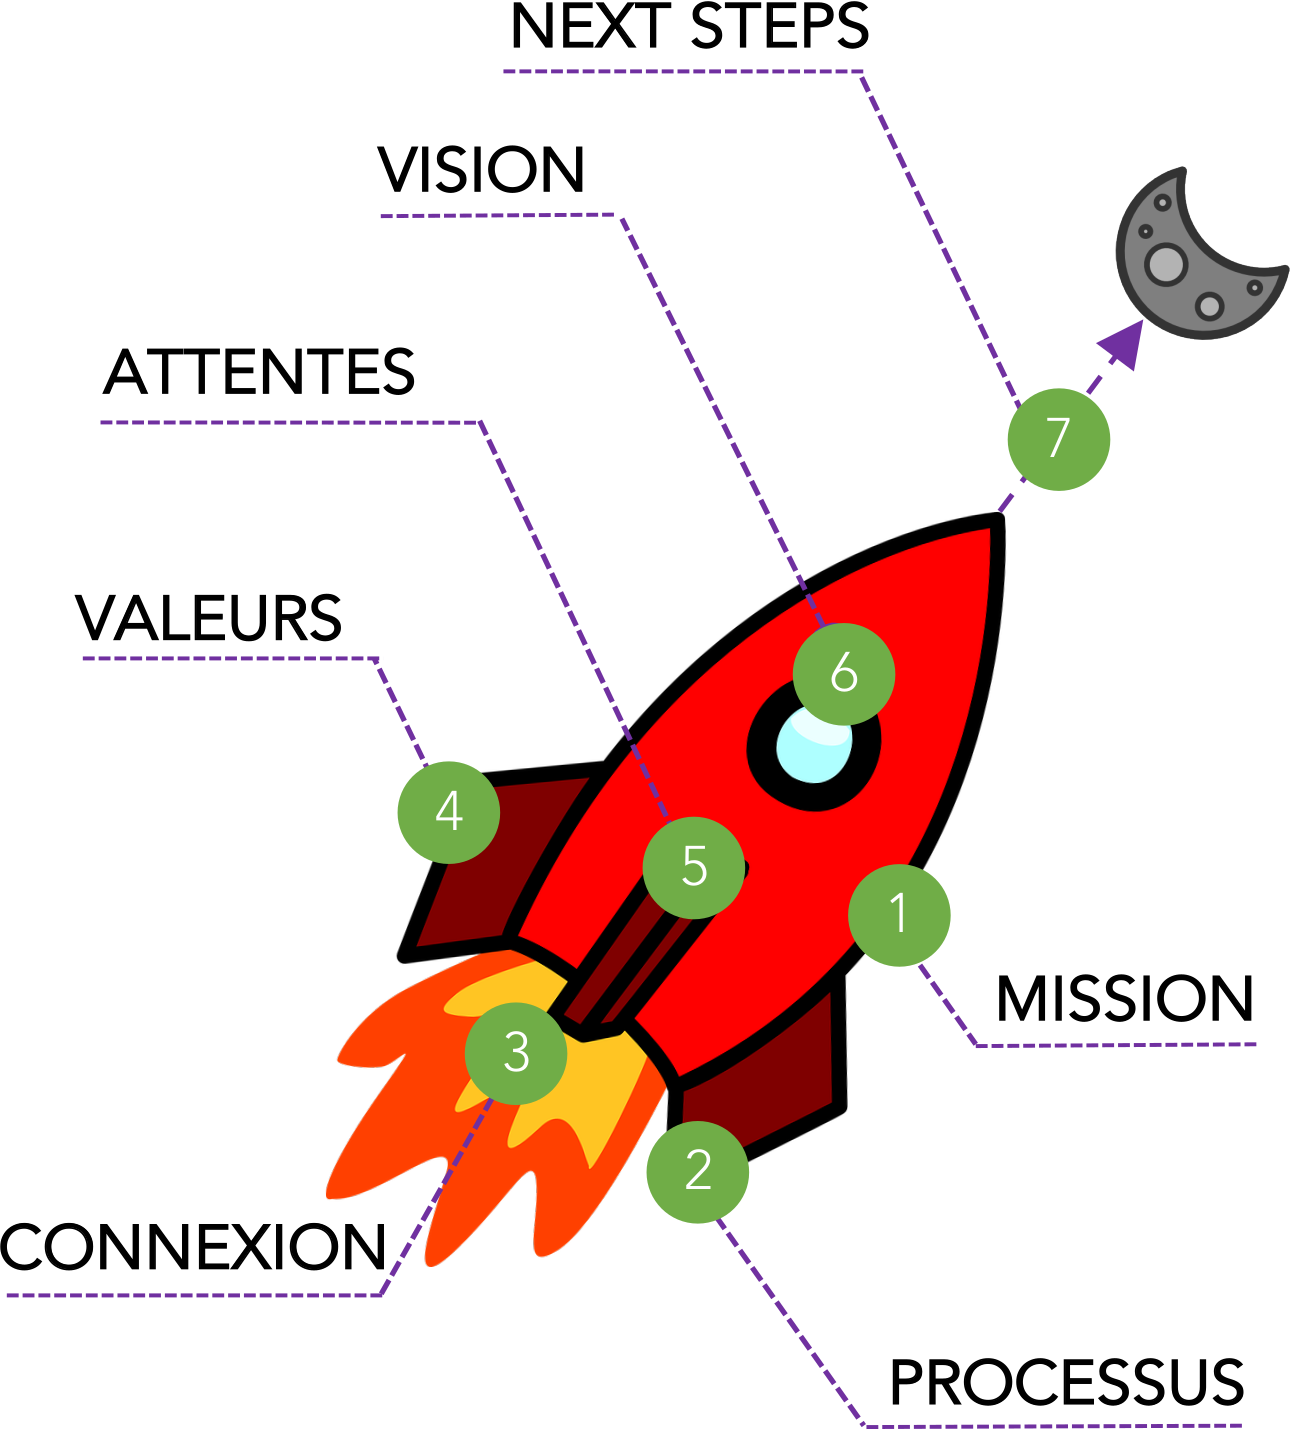
\includegraphics[width=4in]{guide_fusee_definition.png}
\caption{Guide fusée de CimarLab}
\label{fig:guide_fusee}
\end{figure}

\subsection{Critères éthiques de GNU concernant l'hébergement de logiciel}

La licence AGPLv3 n’est pas toujours bien respectée~\cite{violation_libre_2017}.

Les critères éthiques concernant l'hébergement de logiciel~\cite{gnu_critere_hebergement_2022} doivent être accessibles sur les projets de réseau d’entraide. Un guide avec des critères mesurables pour les services destinées à tous ceux qui veulent utiliser un service pour héberger publiquement du code source libre, ainsi qu'éventuellement des programmes exécutables. Ces critères se concentrent sur la protection de la vie privée, le fonctionnement sans JavaScript non libre\footnote{\url{https://www.fsf.org/campaigns/freejs}} , la compatibilité avec les licences à copyleft et leur philosophie, et l'absence de discrimination contre les utilisateurs, quels qu'ils soient.  Les questions à répondre : 

\begin{enumerate}
    \item Est-ce que l'hébergeur fournit l'accès au code source des programmes qu'il héberge?
    \item Est-ce que l'hébergeur permet la redistribution des copies des programmes qu'il héberge?
    \item Est-ce que l'hébergeur permet aux utilisateurs d'apporter des modifications aux programmes qu'il héberge et de les partager avec la communauté?
    \item Est-ce que l'hébergeur impose des restrictions sur l'utilisation ou la redistribution des programmes qu'il héberge?
    \item Est-ce que l'hébergeur respecte les licences de logiciels libres et les droits d'auteur associés aux programmes qu'il héberge?
    \item Est-ce que l'hébergeur fournit des informations sur les licences de logiciels libres et les droits d'auteur associés aux programmes qu'il héberge?
    \item Est-ce que l'hébergeur respecte la vie privée et la sécurité des utilisateurs des programmes qu'il héberge?
    \item Est-ce que l'hébergeur fournit un support et une assistance adéquats aux utilisateurs des programmes qu'il héberge?
\end{enumerate}

\section{Poïèse}

\subsection{Définition de la poïèse}

La poïèse (ou poïesis) est un terme d'origine grecque qui désigne le processus créatif de fabrication, de production ou de création. Il est souvent utilisé dans le contexte de l'art et de la littérature pour décrire le processus de création d'une œuvre, que ce soit un poème, une pièce de théâtre, un roman ou une peinture.

Dans ce contexte, la poïèse est considérée comme un processus actif et dynamique, impliquant l'imagination, l'inspiration, la créativité et la maîtrise technique. Elle implique souvent un certain niveau d'engagement personnel et émotionnel de la part de l'artiste\label{poiese_artise} ou du créateur.

En dehors de l'art, le terme poïèse peut également être utilisé pour décrire tout processus de création ou de production, y compris dans des domaines tels que la science, la technologie ou l'industrie.

\subsection{Allopoïèse}

Un système qui développe\footnote{production/fabrication : Utiliser sans limitation, Modifier pour adapter, Étudier pour comprendre le fonctionnement et Copier pour reproduire.} quelques choses avec des composantes externes.

«L'allopoïèse est le processus par lequel un système produit quelque chose qui n'est pas le système lui-même. Ceci est le contraire de l'autopoïèse.[...] La plupart des processus de production industrielle sont allopoïétiques : une chaîne de montage peut produire des voitures mais pas les machines utilisées dans cette forme de production. [...] La reproduction n'est pas une auto-production.»~\cite{wiki_allopoiesis_2018}~\cite{vuc_allopoiesis_2018}


% «une définition qui est proche de celle d’une machine abstraite et qui décrit la machine comme autopoïétique, autoproductrice d’elle-même et reproduisant en permanence ses composantes tel un système sans input ni output. Varella développe assez loin cette théorie. Il oppose dans sa conception, l’autopoïèse qu’il rapporte essentiellement aux êtres vivants biologiques, à une allopoïèse où la machine va chercher ses composantes à l’extérieur d’elle-même. En fait, dans son concept d’allopoïèse il range les systèmes sociaux, les machines techniques et, pour finir, tous les systèmes machiniques qui ne sont pas des systèmes vivants.»
% «Les machines allopoïétiques se trouvent toujours en adjacence à des machines autopoïétiques et il faut donc prendre en considération les agencements qui les font vivre ensemble.»
% Citer ce document / Cite this document :
% Guattari Félix. À propos des machines. In: Chimères. Revue des schizoanalyses, N°19, printemps 1993. pp. 85-96 ;
% doi : https://doi.org/10.3406/chime.1993.1881
% https://www.persee.fr/doc/chime_0986-6035_1993_num_19_1_1881


\subsection{Autopoïèse}

Un système qui se développe par soi même avec seulement ses composantes internes.

«L'autopoïèse est la propriété d'un système de se produire lui-même, en permanence et en interaction avec son environnement, et ainsi de maintenir son organisation (structure) malgré son changement de composants (matériaux) et d'informations (données).[...]le maintien de sa propre organisation (auto-production)»~\cite{wiki_autopoiesis_2022}.

Le maintien de sa propre organisation signifie l'auto-production, voir exemple illustratif auto-reproducteur~\ref{exemple_illustratif_auto_reproducteur}.

Un système est de l'autopoïèse~\cite{tatsuya_computational_autopoiesis_2000} dans le contexte qu'il est : 
\begin{enumerate}
    \item \textbf{Autonome} : il doit être capable d'apporter des changements variés pour maintenir son organisation;
    \item \textbf{Individuel} : il doit être indépendant dans sa définition, par sa prise de décision par rapport aux observateurs externes, en reproduisant à répétition et maintenant son organisation;
    \item \textbf{Connaissant et établis ses limites} : il doit être capable d'établir ses limites dans son processus de reproduction par lui même sans se faire affecter des limites établis par les observateurs externes;
    \item \textbf{Absent d'entrant et de sortant} : Les stimulis externes doivent être interprété dans un contexte d'observation pour en retirer de l'amélioration continue, elles ne doivent pas impacter la maintenance de l'organisation directement, mais son évolution doit en prendre compte.
\end{enumerate}

Le concept de vue sur les entrants et sortants d'un système est une perception des observateurs externes et ne clarifie pas l'organisation ou les opérations de production du système. 

% TODO à valider : Ainsi, le système va opérer sans s'ajuster lui-même en rapport avec son état et le stimulis externe.

% TODO Alors comment fait-il pour se produire lui même en interaction avec son environnement s'il n'a pas d'entrant et sortant?

La conception d'un système autopoïèse\cite{tatsuya_computational_autopoiesis_2000} devrait comporter les points suivants : 

\begin{enumerate}
    \item Les composantes du système sont déterminé par les opération du système;
    \item Les opérations du système sont produites avant les conditions initiaux;
    \item Les opérations du système sont seulement exécutés pour leur propre réussite et non pour réaliser la production d'un produit;
    \item Dans les opérations du système, ce qui se passent à l'intérieur du système est clairement différent des jugements des observateurs externes.
\end{enumerate}

% TODO La Technopoïèse doit être différent de l'autopoïèse, bien qu'il doit être autonome dans son évolution, il doit suivre des principes moraux et respecter des règles de société.

%  L'autopoïèse s'applique aussi à l'être humain, tant en sociologie\footnote{\url{https://fr.wikipedia.org/wiki/Sociologie}}, la science cognitive\footnote{\url{https://fr.wikipedia.org/wiki/Sciences_cognitives}}, la philosophie\footnote{\url{https://fr.wikipedia.org/wiki/Philosophie}} et la psychopathologie\footnote{\url{https://fr.wikipedia.org/wiki/Psychopathologie}}.

Appliquer l'autopoïèse sur un système est de forcer un changement de point de vue vers l'intérieur du système, puisque l'extérieur est matière à interprétation par la distinction de son environnement. En science naturelle, ce changement de point de vue est difficilement acceptable puisque le point de vue est fait par des observateurs externes.

Des modèles mathématiques sont expliqués dans l'article~\cite{tatsuya_computational_autopoiesis_2000} tel un système de réparation du métabolisme ((M,R) systems), introduit par Rosen, pour démontrer le «Quasi-Autopoietic Systems».
Puis il y a des modèle d'apprentissage automatique qui ont été inspiré de l'autopoïèse pour effectuer des tâches de reconnaissance de formes. Pour pouvoir représenter l'autopoïèse en mathématique ou en modèle informatique, il est nécessaire de trouver un mécanisme d'un système qui crée son espace avec ses limites et son environnement, par soi-même.

% TODO documentation intéressante : https://www.researchgate.net/publication/228784157_A_Computational_Aspect_of_Autopoiesis

\subsection{Sympoïèse}

Un système qui développe en collectivité. Caractéristique d'une technologie qui fait de la poïèse.

La sympoïèse est un concept utilisée en écologie et en théorie des systèmes pour décrire les processus de production collective et collaborative dans les écosystèmes. Elle se distingue de l'autopoïèse, qui est le processus par lequel un système produit et reproduit ses propres composants de manière autonome. Par exemple, les coraux sont des collectifs d'organismes en interaction qui produisent des structures complexes telles que des récifs, qui ont des effets bénéfiques sur l'écosystème dans son ensemble.

«La nature est une puissance d’engendrement qui surgit et s’autoproduit. Donna Haraway a récemment proposé de remplacer le concept "d’autoproduction" par celui de "sympoïèse" qui désigne la coproduction du milieu par des espèces en interrelations plutôt que l’activité autonome de certains organismes isolés.»~\cite{guillibert:tel-02929676}

\subsection{Technopoïèse}

Un système technologique qui développe. Caractéristique d'une technologie qui fait de la poïèse.

% Un système technologique qui travaille pour la poïèse en mettant en place plusieurs caractéristiques, par exemple : l'«Allo» et l'«Auto».

La technologie est là pour assister l'utilisateur et l'accompagner dans l'évolution de celle-ci. «Parce que l’appareil prend place entre la manifestation de l’œuvre et le travail de l’artiste en les découplant, en leur imposant une langue intermédiaire qui code puis décode. L’artiste produit des lignes de code, que la technologie intègre pour fournir à l’œuvre la source de sa manifestation : elle sépare ontologiquement\footnote{Une ontologie est une représentation formelle et explicite de la connaissance d'un domaine, qui spécifie les concepts, les relations et les entités qui existent dans ce domaine et comment ils sont interconnectés.} le travail de l’un et son résultat dans l’autre.»~\cite{artiste_techno_conf_2012} L'artiste~\footnote{Voir l'artiste de la «Définition de la poïèse»~\ref{poiese_artise}} ici signifie un programmeur informatique dans un processus créatif de fabrication, de production ou de création sur des technologies.

Pour éviter que la machine prend le dessus, il faut l'orienter vers la technopoïèse. «Si la technologie est un médium parasite, alors ne suffit-il pas de compter sur la charge poïétique du médium primaire, pour conserver à la poïèse ses caractères nécessaires – et imaginer l’art technologique comme un art d’abord, agrémenté, partiellement seulement, de technologie?»~\cite{artiste_techno_conf_2012} % Cette machine doit être libre pour respecter l'humain. % TODO référence machine libre respect humain

%«Our main claim in this study is to underline that the biopoetic process organizing technopoiesis involves at least four levels, with emergences and constrains between the levels. Furthermore, we see technopoiesis as the dynamics between these four levels based on mechanisms expressing the relation between biology, poetics and external representations that cognitively and socio-culturally ground the evolution of technology.»~\cite{10553_41343}

La relation entre la sympoïèse et la technopoïèse permettrait de concevoir des technologies plus durables et écologiquement responsables, qui favorisent la production collective et collaborative dans les écosystèmes.

Ainsi, le terme «technopoïèse» fait référence à la capacité de l'humanité à créer et à façonner la technologie pour répondre à ses besoins et à ses désirs. 

\subsection{Auto-technopoïèse}

% TODO source chatgpt

% L'auto-technopoïèse étend cette idée, de la technopoïèse, en suggérant que les systèmes technologiques peuvent devenir autonomes et se réguler eux-mêmes sans l'intervention humaine.

L'auto-technopoïèse est un concept qui décrit la capacité des systèmes technologiques à s'auto-organiser et à s'auto-réguler. Plus précisément, l'auto-technopoïèse se réfère à la capacité des systèmes technologiques à maintenir leur propre structure, leur fonctionnement et leur évolution, en utilisant des mécanismes internes de régulation et d'adaptation.

% Le terme "technopoïèse" fait référence à la capacité de l'humanité à créer et à façonner la technologie pour répondre à ses besoins et à ses désirs. L'auto-technopoïèse étend cette idée en suggérant que les systèmes technologiques peuvent devenir autonomes et se réguler eux-mêmes sans l'intervention humaine.

% Un exemple d'auto-technopoïèse est l'Internet, qui est un système complexe de réseaux informatiques interconnectés à l'échelle mondiale. L'Internet est capable de s'auto-réguler et de s'adapter à des changements dans son environnement, tels que l'augmentation du trafic de données ou les pannes de serveurs. Cela est rendu possible grâce à des mécanismes internes de régulation, tels que les protocoles de communication standardisés et les systèmes de routage dynamique.

% En résumé, l'auto-technopoïèse est un concept qui décrit la capacité des systèmes technologiques à s'auto-organiser et à s'auto-réguler. Cette capacité est de plus en plus importante à mesure que les systèmes technologiques deviennent plus complexes et interconnectés.

Pour faire des améliorations technologiques dans la société, sur des réseaux d'entraide, il faut orienter l'auto-technopoïèse dans de la R\&D~\cite{innovation_complex_social_system_2010} orienté aux besoins technologiques dans la gestion de cas d'urgence humanitaire, par exemple le «mouvement des villes en transition»\footnote{\url{https://fr.wikipedia.org/wiki/Ville_en_transition}}, en lien avec la sympoïèse.

% https://transitionlibre.ca

% Référence : 
% Teubner, G. (1993). Autopoietic law: A new approach to law and society. Walter de Gruyter.
% Luhmann, N. (1986). The autopoiesis of social systems. John Wiley & Sons.
% Castells, M. (1996). The rise of the network society. Blackwell Publishers.
% Ahrweiler, P. (2012). Innovation in complex social systems. Routledge.

\section{sécurité}

«La morale de l'article~\cite{thompson_trusting_1984}, alors, est assez simple : il est impossible de fonctionner sans faire confiance à quelqu'un. À moins que vous n'ayez écrit tout le code (et je veux dire TOUT le code) vous-même, vous devrez faire confiance à la sécurité d'une partie du processus de traitement du programme.»~\cite{discussion_reflection_trusting_2020} L'automate codeur doit apprendre à développer toute les étapes de programmation sur une machine.

«Cela suggère que tant que nous ne sommes pas en mesure de rétroconception\footnote{Faire de la rétro-ingénierie sur un développement.} et de contrôler pleinement la fonctionnalité des réseaux neuronaux, il existera un risque inhérent. Même si nous parvenons à résoudre le problème d'alignement et à rendre l'IA conviviale pour l'homme, les attaquants qui obtiennent un accès en écriture aux poids\footnote{Un poids est la valeur numérique d'une neurone dans un réseau de neurones.} pourront implanter leurs portes dérobées.»~\cite{discussion_reflection_trusting_ia_2023} L'automate doit être en mesure de comprendre le fonctionnement d'une machine pour l'étudier.


Problème de sécurité lorsque utilisation de fausse représentation de la licence libre.
% YODO ref agpl sécurité